%Version 3 October 2023 template; build with the official sn-jnl.cls
\documentclass[pdflatex,sn-mathphys-num,iicol]{sn-jnl}
\usepackage{graphicx}
\usepackage{multirow}
\usepackage{amsmath,amssymb,amsfonts}
\usepackage{amsthm}
\usepackage{mathrsfs}
\usepackage{xcolor}
\usepackage{textcomp}
\usepackage{booktabs}
\usepackage{url}
\theoremstyle{thmstyleone}
\newtheorem{theorem}{Theorem}
\newtheorem{proposition}[theorem]{Proposition}
\theoremstyle{thmstyletwo}
\newtheorem{remark}{Remark}
\newcommand{\E}{\mathbb{E}}
\renewcommand{\Pr}{\mathbb{P}}
\raggedbottom
\begin{document}
\title[Trust confidence sets]{Trust confidence sets: statistical inference for selecting models under several trustworthiness criteria}
\author*[1]{\fnm{Vinh} \sur{Dang}}\email{vinh.dang3@rmit.edu.vn}
\affil*[1]{\orgname{RMIT University Vietnam}, \country{Vietnam}}
\abstract{Trustworthy machine learning is assessed on several criteria at once: error, group fairness, calibration and robustness. Candidate models are usually compared through point estimates on one finite test sample, and the winner or the Pareto front of those estimates is reported as if it were a population fact. We describe a trust confidence set (TCS), a data-dependent set of models that contains every population-nondominated model with probability at least $1-\alpha$, asymptotically. It uses a paired bootstrap of one shared test sample, studentised pairwise differences, an intersection--union step across criteria and a maximum over rivals, so it accepts criteria such as calibration error and fairness gaps. In simulation, the TCS retained all nondominated models in at least 99.7\% of replications, whereas the Pareto front of point estimates did so in 34--42\%, and the TCS excluded more dominated models than a Bonferroni box procedure. Validated against a large held-out reference on Adult and Bank Marketing, the point-estimate Pareto front recovered the reference set in 10--76\% of test samples of 500--5000 rows and the composite-score winner matched in 13--75\%; the TCS always retained the reference set but excluded almost no model, because few were truly dominated. Step-down, equivalence margins and a refit bootstrap added little.}
\keywords{trustworthy machine learning, model selection, Pareto dominance, confidence set, bootstrap, algorithmic fairness}
\maketitle
\section{Introduction}
Predictive accuracy is no longer the only quantity of interest when a machine learning model is deployed. Regulators, auditors and practitioners ask whether the model is accurate, whether its errors are distributed fairly across groups, whether its probabilities are calibrated and whether its output is stable under perturbation of the input. The Special Issue on Statistics for Data Science and AI frames this agenda as making models ``accurate, explainable, robust and fair'', and asks for methods that measure trustworthiness in real applications. A growing literature supplies the measures: equality of opportunity \cite{hardt2016}, expected calibration error \cite{guo2017}, and rank-based families of metrics for accuracy, explainability, robustness and fairness \cite{giudici2024robust,babaei2025rgb,wu2026safe}.

What this literature does not supply is an inferential layer for the \emph{comparison} of models on these measures. A trust measure computed on a test sample is an estimate. Two candidate models may differ by less than the sampling noise on one criterion, and may reverse order on another. When the selection rule is ``smallest composite score'' or ``member of the Pareto front of the estimates'', its output is a random set or a random index, and the report rarely says how variable that is. The problem is old in forecasting and econometrics, where the reality-check and superior-predictive-ability tests \cite{white2000,hansen2005spa} and the model confidence set \cite{hansen2011mcs} replace a single winner by a set that is guaranteed to contain the best model with stated confidence. Those tools compare models under one loss, or under a class of losses applied to a single forecast-error series \cite{arvanitis2021,jin2017}. Trustworthiness is a vector of heterogeneous criteria, each a different functional of the data.

\paragraph{Contribution.} Set-wise confidence guarantees for the Pareto set of a finite list already exist outside machine-learning evaluation (Section~\ref{sec:related}). We adapt this idea to the evaluation of trained models on a common test sample. We define a population notion of nondominated models under a vector of trust criteria and a \emph{trust confidence set} (TCS) built from a paired, studentised bootstrap of pairwise differences, which contains all such models with asymptotic probability at least $1-\alpha$ and accepts any criteria that are functionals of the empirical distribution. We (i) prove asymptotic control under bootstrap consistency, (ii) show by simulation that the Pareto front of point estimates fails badly at the same task, (iii) compare the TCS with a marginal-box procedure and show where the pairing buys power, (iv) examine four extensions and report that two of them add little, (v) check the procedures against a large held-out reference on real models and data, and (vi) apply the method to two public benchmarks to show how many models survive. We also give a Pareto-membership probability as a descriptive companion, a device already used descriptively elsewhere.

\section{Related work}\label{sec:related}
\paragraph{Statistical comparison of learners.} Significance testing for classifiers on one or several datasets is well established \cite{dietterich1998,demsar2006}, and Bayesian alternatives have been argued to be more informative than null-hypothesis tests \cite{benavoli2017}. Bouthillier et al.\ \cite{bouthillier2021} show that benchmark conclusions depend on several sources of variance (data sampling, initialisation, hyper-parameter search), and that ignoring them inflates claimed improvements. These works compare models on one performance metric.

\paragraph{Confidence sets for model selection.} Hansen, Lunde and Nason \cite{hansen2011mcs} introduce the model confidence set, a set of models that contains the best model with a given probability and that grows when the data are uninformative. The tests of White \cite{white2000} and Hansen \cite{hansen2005spa}, and the step-down multiple-testing framework of Romano and Wolf \cite{romano2005}, supply the bootstrap machinery for maxima of studentised statistics over many comparisons. Our construction borrows this machinery but targets nondominance in a vector of criteria rather than minimality of one loss. The multi-loss extensions of the superior-predictive-ability test \cite{arvanitis2021,jin2017} range over classes of losses applied to one error series per model, which is a different structure from a finite vector of unrelated criteria.

\paragraph{Confidence statements for Pareto sets.} Several literatures give set-wise guarantees for the Pareto set of a finite list. In bandit theory, fixed-confidence Pareto set identification returns the Pareto-optimal arms with probability at least $1-\delta$ through adaptive sampling \cite{auer2016,kone2023,crepon2024}; in ranking and selection, Andrad\'ottir and Lee \cite{andradottir2021} give a procedure with a guaranteed probability of correct selection of the Pareto set; SPRINT-Race \cite{zhang2018sprint} races candidate learners to a Pareto-optimal set under a sequential likelihood-ratio test. The closest statement in logic is the one-shot screening of simulated systems by Zhao and Eckman \cite{zhao2026}, a recent preprint: a finite list, a guarantee $\Pr(\text{efficient set}\subseteq S)\ge1-\alpha$, and a rule that retains a system unless it is certifiably dominated, implemented with Bonferroni or \v{S}id\'ak confidence boxes. An R package, \texttt{paretoinfer} \cite{paretoinfer}, reports a ``plausible Pareto set'' of alternatives not certified as dominated, from anytime-valid confidence sequences for bounded outcomes. These works differ from ours in the object they resample (marginal boxes or sequential draws, not the pairwise differences on one shared test sample), in the dominance relation (weak Pareto dominance, against strict dominance here) and in the criteria they cover (means or bounded outcomes, not calibration error or fairness gaps). Auerbach et al.\ \cite{auerbach2024} combine intersection--union testing and a bootstrap to test whether one algorithm can be improved in fairness without losing on other objectives; they test a single algorithm rather than return a set. We found no work that returns a confidence set of non-dominated models from a fixed list of trained models on a shared test sample for trust criteria, but the area is moving fast and our search was not exhaustive.

\paragraph{Uncertainty in fairness and trust measures.} Group-fairness estimates have large variance for small groups. Miller et al.\ \cite{miller2021} propose model-based estimators and an approximate bootstrap for subpopulation metrics, and Ferrara et al.\ \cite{ferrara2025} derive a central limit theorem for statistical parity difference with a Wald test and a Bayesian estimator for small intersectional groups. Those papers quantify the uncertainty of \emph{one} fairness metric for \emph{one} model. We use bootstrap standard errors for pairwise differences of arbitrary criteria across models.

\paragraph{Model multiplicity.} Underspecification \cite{damour2022} and predictive multiplicity \cite{marx2020} document that many models with near-identical accuracy can differ in fairness, robustness and individual predictions. This is the setting in which a point-estimate winner is least reliable, and in which the TCS is meant to report which differences can and cannot be resolved with the available test data.

\paragraph{Trust metrics in this journal.} Recent contributions to the \emph{International Journal of Data Science and Analytics} include robustness measures for linear and nonlinear models \cite{giudici2024robust}, fairness metrics for credit lending \cite{wu2026safe}, and evaluation of imputation methods by downstream predictive performance \cite{nikitina2026}. The Rank Graduation Box \cite{babaei2025rgb} unifies accuracy, explainability, robustness and fairness through rank-based measures. Our method is complementary: it can take any of these measures as a coordinate of the criterion vector (Section~\ref{sec:ext}) and says how much of a difference between models is resolved by the data.

\section{Method}
\subsection{Setting and target}
Let $\mathcal{M}=\{1,\dots,M\}$ be candidate models, already trained, and let $D=\{z_i\}_{i=1}^n$ be a test sample of independent instances. For each model $m$ and criterion $k=1,\dots,K$ let $\hat c_{mk}=\phi_k(\hat F_m)$ be an estimate of $\mu_{mk}=\phi_k(F_m)$, where $F_m$ is the population law of the (instance, prediction, perturbed prediction, group) record produced by model $m$ and $\phi_k$ is a smooth functional. All criteria are oriented so that smaller is better (error, equalised-odds gap, calibration error, performance loss under perturbation). Inference is conditional on the trained models; Section~\ref{sec:disc} discusses training variability.

\begin{table}[t]\centering
\caption{Criteria used in the experiments. Each is a functional of the empirical distribution of one model's test records.}
\begin{tabular}{lp{5.4cm}}\toprule
Criterion & Definition\\\midrule
Error & misclassification rate\\
EO gap & $\max\{|\mathrm{TPR}_0-\mathrm{TPR}_1|,|\mathrm{FPR}_0-\mathrm{FPR}_1|\}$ across the two groups \cite{hardt2016}\\
ECE & 10-bin expected calibration error of the predicted probability \cite{guo2017}\\
Noise drop & error on the perturbed test sample minus error on the clean sample\\\bottomrule
\end{tabular}
\end{table}

\paragraph{Definition.} Model $m$ is \emph{strictly dominated} by model $j$ if $\mu_{mk}>\mu_{jk}$ for every $k$. The population nondominated set is $\mathcal{P}_0=\{m:\ \text{no } j \text{ strictly dominates } m\}$. This definition is deliberately the weakest notion of domination: a model tied with a rival on a single criterion belongs to $\mathcal{P}_0$. It is the notion for which an exclusion can be certified by a test, since declaring $m$ worse requires evidence of difference on \emph{every} criterion.

\subsection{Procedure}
Let $d_{mjk}=\hat c_{mk}-\hat c_{jk}$ (positive means $m$ is worse). Draw $B$ paired bootstrap samples of the test instances, applying the same resample to all models, and recompute all estimates to obtain $\hat c^{*b}_{mk}$. With $d^{*b}_{mjk}=\hat c^{*b}_{mk}-\hat c^{*b}_{jk}$ and $\hat s_{mjk}$ the bootstrap standard deviation of $d^{*b}_{mjk}$:
\begin{enumerate}
\item the studentised difference is $t_{mjk}=d_{mjk}/\hat s_{mjk}$ and the centred bootstrap version is $t^{*b}_{mjk}=(d^{*b}_{mjk}-d_{mjk})/\hat s_{mjk}$;
\item the dominance statistic of model $m$ is $S_m=\max_{j\ne m}\min_{k} t_{mjk}$ (an intersection--union statistic across criteria, a maximum over rivals);
\item the critical value $\hat q_{1-\alpha}$ is the $(1-\alpha)$-quantile over $b$ of $\max_{m\ne j,\,k} t^{*b}_{mjk}$;
\item $\mathrm{TCS}_{1-\alpha}=\{m: S_m\le \hat q_{1-\alpha}\}$.
\end{enumerate}
A pair $(m,j)$ with $\hat s_{mjk}=0$ (identical predictions on criterion $k$) is assigned $t_{mjk}=0$.

\begin{proposition}\label{prop:cov}
Suppose that, jointly over $(m,j,k)$, the bootstrap law of $\hat s_{mjk}^{-1}(d^{*}_{mjk}-d_{mjk})$ is consistent for the law of $\hat s_{mjk}^{-1}(d_{mjk}-\delta_{mjk})$ with $\delta_{mjk}=\mu_{mk}-\mu_{jk}$, and that the limit has a continuous distribution function at its $(1-\alpha)$-quantile. Then $\limsup_{n\to\infty}\Pr(\mathcal{P}_0\not\subseteq \mathrm{TCS}_{1-\alpha})\le\alpha$.
\end{proposition}
\begin{proof}[Sketch]
Fix $m\in\mathcal{P}_0$. For every rival $j$ some criterion $k(j)$ satisfies $\delta_{mjk(j)}\le0$, so $t_{mjk(j)}\le z_{mjk(j)}:=\hat s_{mjk(j)}^{-1}(d_{mjk(j)}-\delta_{mjk(j)})$. Hence $S_m\le\max_j t_{mjk(j)}\le\max_{j,k}z_{mjk}\le Z:=\max_{m',j,k}z_{m'jk}$. The model $m$ is excluded only if $S_m>\hat q_{1-\alpha}$, which requires $Z>\hat q_{1-\alpha}$. By the consistency assumption, $\hat q_{1-\alpha}$ converges to the $(1-\alpha)$-quantile of the limit law of $Z$, so $\Pr(Z>\hat q_{1-\alpha})\to\alpha$. A union over $m\in\mathcal{P}_0$ is not needed because the bound on $Z$ is common to all models.
\end{proof}

\begin{remark}[Conservativeness]
The critical value takes a maximum over criteria rather than a minimum because a model in $\mathcal{P}_0$ may be tied with a rival on a single criterion while clearly worse on the others (the least favourable configuration of an intersection--union test). Using the minimum under a global null that sets all differences to zero gives a smaller critical value; in a preliminary run of the simulation design of Section~\ref{sec:sim}, that variant retained all of $\mathcal{P}_0$ in only 85--94\% of replications when $\rho=0$, below the nominal level, which is why it is not used. The price is lower power; sharper step-down variants \cite{romano2005} are a natural extension.
\end{remark}

\begin{remark}[Companion indices]
Two descriptive quantities accompany the set. The Pareto-membership probability $\hat\pi_m=B^{-1}\sum_b \mathbf{1}\{m \text{ is on the Pareto front of } \hat c^{*b}\}$, and, for any scalarisation (here an equal-weight sum of criteria divided by their across-model standard deviation), the bootstrap distribution of the rank and of the arg-min. These carry no coverage guarantee; they show how unstable a point-estimate decision is.
\end{remark}

\section{Simulation}\label{sec:sim}
\paragraph{Design.} There are $M=8$ models and $K=3$ criteria. Population means (smaller is better) for models 0--3 are $(0.10,0.10,0.30)$, $(0.30,0.10,0.10)$, $(0.10,0.30,0.10)$ and $(0.20,0.20,0.20)$; with $\mu_3=(0.20,0.20,0.20)$ and margin $\delta\in\{0.02,0.05\}$, model 4 is $\mu_3+\delta(1,1,1)$ and model 5 is $\mu_3+2\delta(1,1,1)$ (both strictly dominated by model 3), model 6 is $\mu_3+\delta(1,1,0)$ (tied with model 3 on criterion 3, hence in $\mathcal{P}_0$) and model 7 is $\mu_3+\delta(1,1,-1)$ (a trade-off, in $\mathcal{P}_0$). Per-instance values are Gaussian with standard deviation $0.15$, correlation $\rho\in\{0,0.5\}$ between criteria within a model and $0.5$ between models. Test sizes are $n\in\{200,500,2000\}$, with 400 replications per cell, $B=300$ bootstrap samples and $\alpha=0.05$. The naive competitor is the Pareto front of the point estimates. Two outcomes are recorded: whether \emph{all} models of $\mathcal{P}_0$ are retained, and the share of strictly dominated models that are excluded.

\paragraph{Results.} Table~\ref{tab:sim} and Figure~\ref{fig:sim} give the results. The TCS retained all models of $\mathcal{P}_0$ in at least 99.75\% of replications in every cell; the sampling error of an estimated proportion with 400 replications is about one percentage point, and the proportions are well above the nominal 95\%, which is consistent with the conservativeness discussed above. The naive Pareto front retained all of $\mathcal{P}_0$ in 33.5--42.3\% of replications, and the proportion did not improve with $n$: the tied model 6 is on the estimated front only when sampling noise happens to favour it on criterion 3. The naive front excluded dominated models more often than the TCS at small $n$ (for example $n=200,\delta=0.02$: 0.97 versus 0.15--0.23), which is exactly the behaviour of an unfounded decision rule. The TCS exclusion share rises with $n$ and $\delta$ and reaches one at $n=2000$ (0.995 or higher in all cells).

\begin{table*}[t]\centering\small
\caption{Monte Carlo results (400 replications per row). Retention: probability that all population-nondominated models are retained (nominal 0.95). Exclusion: share of strictly dominated models removed. TCS size: mean number of models retained (population nondominated: 6).}\label{tab:sim}
\begin{tabular}{rrrrrrrr}\toprule
$n$ & $\delta$ & $\rho$ & \multicolumn{2}{c}{Retention} & \multicolumn{2}{c}{Exclusion} & TCS size \\
 & & & TCS & Naive & TCS & Naive & \\\midrule
200 & 0.02 & 0.0 & 1.000 & 0.422 & 0.15 & 0.97 & 7.69 \\
200 & 0.02 & 0.5 & 0.998 & 0.362 & 0.23 & 0.98 & 7.53 \\
200 & 0.05 & 0.0 & 1.000 & 0.385 & 0.87 & 1.00 & 6.25 \\
200 & 0.05 & 0.5 & 0.998 & 0.410 & 0.92 & 1.00 & 6.15 \\
500 & 0.02 & 0.0 & 1.000 & 0.355 & 0.51 & 1.00 & 6.97 \\
500 & 0.02 & 0.5 & 1.000 & 0.335 & 0.57 & 1.00 & 6.86 \\
500 & 0.05 & 0.0 & 0.998 & 0.380 & 1.00 & 1.00 & 6.00 \\
500 & 0.05 & 0.5 & 1.000 & 0.352 & 1.00 & 1.00 & 6.00 \\
2000 & 0.02 & 0.0 & 1.000 & 0.352 & 0.99 & 1.00 & 6.01 \\
2000 & 0.02 & 0.5 & 1.000 & 0.388 & 1.00 & 1.00 & 6.01 \\
2000 & 0.05 & 0.0 & 1.000 & 0.362 & 1.00 & 1.00 & 6.00 \\
2000 & 0.05 & 0.5 & 1.000 & 0.355 & 1.00 & 1.00 & 6.00 \\
\bottomrule\end{tabular}
\end{table*}
\begin{figure*}[t]\centering
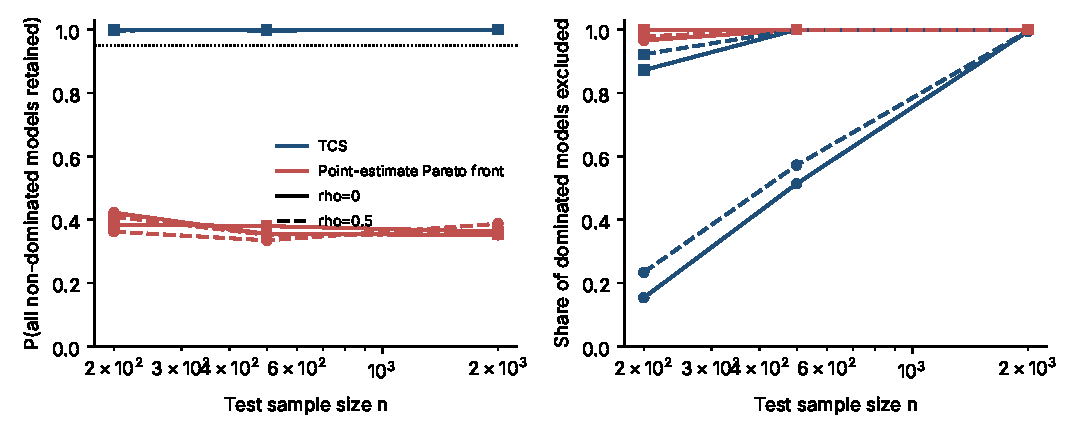
\includegraphics[width=0.9\textwidth]{fig_simulation}
\caption{Retention (left) and exclusion (right) as a function of test size. Blue: TCS. Red: Pareto front of point estimates. Solid: $\rho=0$; dashed: $\rho=0.5$; circles: $\delta=0.02$; squares: $\delta=0.05$.}\label{fig:sim}
\end{figure*}

\subsection{Comparison with a marginal-box procedure}\label{sec:box}
To see what the paired bootstrap adds, we implemented a box procedure in the spirit of Zhao and Eckman \cite{zhao2026}; this is our own implementation of a generic box rule, not their code. Two-sided normal intervals at level $\alpha/(MK)$ are computed for every model and criterion, and model $m$ is excluded if some rival's upper limit lies below $m$'s lower limit on every criterion. The same data are used, with between-model correlation $r=0.5$ (as in the main design) and $r=0$ (independent models, which removes the benefit of pairing).

Table~\ref{tab:box} shows that both procedures retain the nondominated set in at least 99.7\% of replications. The TCS excludes many more dominated models: with $r=0.5$ and $n=500$, $\delta=0.02$ it excludes 0.53--0.57 against 0.03--0.10; at $n=2000$ the figures are 0.99--1.00 against 0.54--0.60. When models are independent the gap narrows (0.24--0.33 against 0.05--0.10 at $n=500$, $\delta=0.02$) but does not vanish, which indicates that studentising pairwise differences and taking a maximum over triples is less wasteful than a Bonferroni split over $MK$ intervals. The size of the gain depends on how strongly models' errors co-vary on a shared test sample, which in practice is usually strong.

\begin{table*}[t]\centering\small
\caption{Retention and exclusion for the TCS and the Bonferroni box procedure (300 replications per row). $r$: correlation between models' per-instance values; $\rho$: correlation between criteria. Retention is the minimum over the two settings of $r$.}\label{tab:box}
\begin{tabular}{rrrrrrrrr}\toprule
$n$ & $\delta$ & $\rho$ & \multicolumn{2}{c}{Retention} & \multicolumn{2}{c}{Exclusion, $r=0.5$} & \multicolumn{2}{c}{Exclusion, $r=0$} \\
 & & & TCS & Box & TCS & Box & TCS & Box \\\midrule
200 & 0.02 & 0.0 & 1.000 & 1.000 & 0.16 & 0.00 & 0.01 & 0.00 \\
200 & 0.02 & 0.5 & 0.997 & 1.000 & 0.25 & 0.00 & 0.05 & 0.00 \\
200 & 0.05 & 0.0 & 1.000 & 1.000 & 0.87 & 0.50 & 0.56 & 0.49 \\
200 & 0.05 & 0.5 & 1.000 & 1.000 & 0.91 & 0.51 & 0.61 & 0.50 \\
500 & 0.02 & 0.0 & 1.000 & 1.000 & 0.53 & 0.03 & 0.23 & 0.05 \\
500 & 0.02 & 0.5 & 1.000 & 1.000 & 0.57 & 0.10 & 0.33 & 0.10 \\
500 & 0.05 & 0.0 & 1.000 & 1.000 & 1.00 & 0.88 & 0.96 & 0.80 \\
500 & 0.05 & 0.5 & 0.997 & 1.000 & 1.00 & 0.88 & 0.97 & 0.81 \\
2000 & 0.02 & 0.0 & 1.000 & 1.000 & 1.00 & 0.54 & 0.76 & 0.55 \\
2000 & 0.02 & 0.5 & 1.000 & 1.000 & 0.99 & 0.60 & 0.82 & 0.61 \\
2000 & 0.05 & 0.0 & 1.000 & 1.000 & 1.00 & 1.00 & 1.00 & 1.00 \\
2000 & 0.05 & 0.5 & 1.000 & 1.000 & 1.00 & 1.00 & 1.00 & 1.00 \\
\bottomrule\end{tabular}
\end{table*}

\subsection{Non-smooth criteria}\label{sec:nonsmooth}
The designs above use criteria that are plain means. We therefore added a simulation with error, 10-bin expected calibration error (ECE) and the equalised-odds gap, the last two being non-smooth (binning, absolute value and a maximum). Covariates are $x\sim N(0,I_5)$, a binary group $g$ has probability 0.3, and $y$ is Bernoulli with a logistic probability in $x$ and $g$. Each of 12 models is a fixed scoring rule $p_m=\sigma(s_m(\beta_m^\top x+o_m g))$ with a random coefficient vector, temperature and group offset, and predicts $\mathbf 1\{p_m>0.5\}$. Population criteria are the plug-in functionals of the population law (fixed bins, same definitions as the estimator), approximated with $2\times10^6$ independent draws, and the population nondominated set is computed from them. Four randomly drawn designs (with $|\mathcal{P}_0|=7,6,8,4$ of 12) were run at $n\in\{500,2000,10000\}$ with 250 replications each and $B=300$ bootstrap samples (multinomial weights). The box procedure uses bootstrap standard errors. In a second run the twelfth model is an exact copy of the first (ties on every criterion; two designs).

Table~\ref{tab:nonsmooth} shows that the TCS retained the population nondominated set in all 250 replications in every cell, which with 250 replications is consistent with true retention of at least about 98.8\% (a one-sided 95\% bound), and the same held in the duplicate-model run (6 cells, 250 replications each). The Pareto front of point estimates retained it in only 1--68\% of replications. The TCS excluded essentially no model at $n=500$ (at most 0.4\%) and few at $n=2000$ (0.5--19\%), so retention at those sizes is largely vacuous: the set is nearly the whole list. At $n=10000$ it excluded 9--69\% of dominated models against 2--34\% for the box procedure, and the ordering of the two procedures matched that of the mean-criteria design. These results show no failure of retention for non-smooth criteria in these designs. They do not establish the nominal level, because the procedure is conservative and the cells where it excludes something are few; the diagnostic power is at $n=10000$.

\begin{table*}[t]\centering\small
\caption{Non-smooth criteria (error, ECE, equalised-odds gap): 12 models, 250 replications per row. Retention: probability that all population-nondominated models are retained. Exclusion: share of dominated models removed. Box: Bonferroni boxes with bootstrap standard errors; Naive: Pareto front of point estimates.}\label{tab:nonsmooth}
\begin{tabular}{rrrrrrrr}\toprule
Design & $|\mathcal{P}_0|$ & $n$ & \multicolumn{3}{c}{Retention} & \multicolumn{2}{c}{Exclusion} \\
 & & & TCS & Box & Naive & TCS & Box \\\midrule
3 & 7 & 500 & 1.000 & 1.000 & 0.084 & 0.00 & 0.00 \\
3 & 7 & 2000 & 1.000 & 1.000 & 0.288 & 0.19 & 0.07 \\
3 & 7 & 10000 & 1.000 & 1.000 & 0.628 & 0.69 & 0.34 \\
4 & 6 & 500 & 1.000 & 1.000 & 0.224 & 0.00 & 0.00 \\
4 & 6 & 2000 & 1.000 & 1.000 & 0.432 & 0.09 & 0.00 \\
4 & 6 & 10000 & 1.000 & 1.000 & 0.624 & 0.39 & 0.20 \\
8 & 8 & 500 & 1.000 & 1.000 & 0.012 & 0.00 & 0.00 \\
8 & 8 & 2000 & 1.000 & 1.000 & 0.060 & 0.01 & 0.00 \\
8 & 8 & 10000 & 1.000 & 1.000 & 0.412 & 0.22 & 0.02 \\
10 & 4 & 500 & 1.000 & 1.000 & 0.200 & 0.00 & 0.00 \\
10 & 4 & 2000 & 1.000 & 1.000 & 0.396 & 0.01 & 0.00 \\
10 & 4 & 10000 & 1.000 & 1.000 & 0.680 & 0.09 & 0.05 \\
\bottomrule\end{tabular}
\end{table*}

\subsection{Validation with a large held-out pool}\label{sec:realval}
The case studies above have no ground truth. To check the procedures against a reference on real models and data, we trained the nine models once and used the large held-out part of each data set (19,537 rows for Adult, 18,085 for Bank Marketing) as a proxy for the population. Reference criteria (error, ECE, equalised-odds gap, noise drop) were computed on the whole pool, and the reference nondominated set $\mathcal{P}_{\mathrm{ref}}$ is the set of models not strictly dominated on the pool. Test samples of $n\in\{500,1000,2000,5000\}$ rows were then drawn from the pool without replacement (200 per cell), and each was analysed as a practitioner would: Pareto front of the point estimates, the model with the smallest equal-weight composite score (criteria scaled by their reference standard deviations), and the TCS with $B=300$. Three settings were used: Adult with sex as the group, Adult with race (non-White against White), and Bank Marketing (age below 30, OpenML version 1, target ``yes'').

Table~\ref{tab:realval} shows the following. (i) The Pareto front of the point estimates retained all of $\mathcal{P}_{\mathrm{ref}}$ in only 10--76\% of samples (about 21\% at $n=500$ on both Adult settings and 10\% on Bank Marketing), and it was too small on average (for example 7.2 models against 8 at $n=500$ on Adult by sex). (ii) The composite-score winner matched the reference winner in 13--25\% of samples on Adult by sex, 38--75\% on Adult by race and 16--38\% on Bank Marketing, with six to nine distinct winners among 200 samples at every size. (iii) The TCS retained all of $\mathcal{P}_{\mathrm{ref}}$ in every sample, but it excluded almost nothing (at most 4\% of the dominated models), so its size was nine of nine. This is close to the truth in these data: the reference sets contain 8, 8 and 7 of 9 models, so at most one or two models can be excluded and the TCS overshoots by one or two while the naive front undershoots and misses members. The reference sets are themselves estimates on a finite pool, the models are fixed, the subsamples are drawn without replacement from the pool (which makes the intervals slightly conservative), and the group definitions are conventions.

\begin{table*}[t]\centering\small
\caption{Validation against a large held-out pool (200 samples per row, nine models, four criteria). Retention: share of samples in which all models of the reference nondominated set were kept. Winner correct: share of samples whose composite-score winner equals the reference winner. Excl.: share of reference-dominated models excluded by the TCS.}\label{tab:realval}
\begin{tabular}{llrrrrrrrr}\toprule
Data & $n$ & \multicolumn{2}{c}{Retention} & \multicolumn{3}{c}{Set size} & Winner & Excl. \\
 & & Naive & TCS & Naive & TCS & Ref. & correct & (TCS) \\\midrule
Adult (sex) & 500 & 0.21 & 1.00 & 7.2 & 9.0 & 8 & 0.13 & 0.00 \\
 & 1000 & 0.36 & 1.00 & 7.4 & 9.0 & 8 & 0.17 & 0.00 \\
 & 2000 & 0.54 & 1.00 & 7.8 & 9.0 & 8 & 0.20 & 0.00 \\
 & 5000 & 0.76 & 1.00 & 8.1 & 9.0 & 8 & 0.25 & 0.01 \\
Adult (race) & 500 & 0.21 & 1.00 & 7.0 & 9.0 & 8 & 0.38 & 0.00 \\
 & 1000 & 0.26 & 1.00 & 7.1 & 9.0 & 8 & 0.48 & 0.00 \\
 & 2000 & 0.36 & 1.00 & 7.3 & 9.0 & 8 & 0.63 & 0.00 \\
 & 5000 & 0.59 & 1.00 & 7.6 & 9.0 & 8 & 0.75 & 0.04 \\
Bank (age) & 500 & 0.10 & 1.00 & 6.2 & 9.0 & 7 & 0.16 & 0.00 \\
 & 1000 & 0.17 & 1.00 & 6.4 & 9.0 & 7 & 0.20 & 0.00 \\
 & 2000 & 0.22 & 1.00 & 6.6 & 9.0 & 7 & 0.28 & 0.00 \\
 & 5000 & 0.47 & 1.00 & 7.2 & 9.0 & 7 & 0.38 & 0.00 \\
\bottomrule\end{tabular}
\end{table*}

\section{Case studies}
\paragraph{Data and models.} We use the Adult census income data (OpenML, version 2; 48,842 records; sensitive attribute: sex, removed from the features) and the German credit data (OpenML, version 1; 1,000 records; group: age below 26, a frequently used convention, with age removed from the features). Each data set is split once with a stratified 60/40 train/test split (seed 0), giving $n_{\text{test}}=19{,}537$ and $400$. Nine models are trained with scikit-learn defaults unless stated: logistic regression, logistic regression with $C=0.01$, decision trees of depth 3 and 12, random forest (200 trees, minimum leaf 3), histogram gradient boosting, 25-nearest neighbours, Gaussian naive Bayes and a two-layer perceptron (64, 32 units, early stopping). Numeric features are standardised and categorical features one-hot encoded. For the noise criterion, numeric test features are perturbed once with Gaussian noise of standard deviation equal to half the training standard deviation. We use $B=1000$ bootstrap samples and $\alpha=0.05$. The fairness measures are used only as an illustration of vector-valued comparison and say nothing about the fitness of these models for decisions about individuals.

\paragraph{Results.} Tables~\ref{tab:adult} and~\ref{tab:german} and Figure~\ref{fig:pp} list the point estimates, the dominance statistics $S_m$ against the critical values ($\hat q=3.58$ for Adult and $3.71$ for German credit), set membership, Pareto-membership probabilities $\hat\pi_m$, and the bootstrap frequency of being the best model by the equal-weight composite score.

\begin{table*}[t]\centering\small
\caption{Adult (sex), $n_{\text{test}}=19{,}537$. $S_m$: dominance statistic (critical value 3.58). Naive: on the Pareto front of the point estimates. $\hat\pi_m$: bootstrap probability of Pareto-front membership. Top-1: bootstrap frequency of minimising the composite score.}\label{tab:adult}
\begin{tabular}{lrrrrrcccr}\toprule
Model & Error & EO gap & ECE & Noise drop & $S_m$ & TCS & Naive & $\hat\pi_m$ & Top-1 \\\midrule
LR & 0.150 & 0.110 & 0.007 & 0.031 & -3.32 & yes & yes & 1.00 & 0.06 \\
LR-strong-reg & 0.152 & 0.157 & 0.015 & 0.023 & -2.37 & yes & yes & 1.00 & 0.00 \\
Tree(d=3) & 0.155 & 0.093 & 0.004 & 0.042 & -1.18 & yes & yes & 0.99 & 0.12 \\
Tree(d=12) & 0.146 & 0.082 & 0.034 & 0.065 & -0.11 & yes & yes & 0.84 & 0.00 \\
RandomForest & 0.136 & 0.121 & 0.020 & 0.039 & -6.63 & yes & yes & 1.00 & 0.00 \\
HistGB & 0.129 & 0.092 & 0.009 & 0.072 & -5.03 & yes & yes & 1.00 & 0.00 \\
kNN(25) & 0.157 & 0.128 & 0.012 & 0.004 & -7.44 & yes & yes & 1.00 & 0.41 \\
NaiveBayes & 0.406 & 0.141 & 0.404 & 0.023 & 0.59 & yes & no & 0.27 & 0.00 \\
MLP & 0.147 & 0.084 & 0.019 & 0.034 & -2.04 & yes & yes & 1.00 & 0.41 \\
\bottomrule\end{tabular}
\end{table*}
\begin{table*}[t]\centering\small
\caption{German credit (age), $n_{\text{test}}=400$. Critical value 3.71.}\label{tab:german}
\begin{tabular}{lrrrrrcccr}\toprule
Model & Error & EO gap & ECE & Noise drop & $S_m$ & TCS & Naive & $\hat\pi_m$ & Top-1 \\\midrule
LR & 0.263 & 0.076 & 0.054 & 0.015 & -0.02 & yes & yes & 0.64 & 0.01 \\
LR-strong-reg & 0.285 & 0.013 & 0.103 & -0.010 & -0.67 & yes & yes & 0.80 & 0.06 \\
Tree(d=3) & 0.297 & 0.035 & 0.035 & -0.005 & -0.84 & yes & yes & 0.94 & 0.04 \\
Tree(d=12) & 0.310 & 0.056 & 0.287 & -0.042 & -0.87 & yes & yes & 0.87 & 0.01 \\
RandomForest & 0.247 & 0.053 & 0.054 & -0.017 & -1.41 & yes & yes & 0.99 & 0.57 \\
HistGB & 0.253 & 0.117 & 0.093 & -0.020 & -0.14 & yes & yes & 0.86 & 0.22 \\
kNN(25) & 0.278 & 0.101 & 0.041 & -0.003 & -0.70 & yes & yes & 0.78 & 0.08 \\
NaiveBayes & 0.297 & 0.092 & 0.229 & 0.008 & 0.51 & yes & no & 0.13 & 0.00 \\
MLP & 0.263 & 0.178 & 0.055 & -0.010 & 0.03 & yes & no & 0.75 & 0.02 \\
\bottomrule\end{tabular}
\end{table*}

On Adult, all nine models are in the TCS: the largest dominance statistic is 0.59 (naive Bayes), far below the critical value. Naive Bayes is clearly worst on error (0.406) and calibration (0.404), yet it is not significantly dominated: its equalised-odds gap (0.141) lies within the range of the other models' gaps (0.082--0.157) while the bootstrap standard deviation of a single gap is about 0.02, and dominance on all four criteria is required. The Pareto front of the estimates has eight members, and the Pareto-membership probabilities are 1.00 for seven models, 0.84 for the depth-12 tree and 0.27 for naive Bayes. The composite-score winner is not identified: the multilayer perceptron, 25-nearest neighbours and the depth-3 tree were best in 41\%, 41\% and 12\% of resamples, and the 95\% bootstrap intervals of the composite rank of the perceptron, kNN and the depth-3 tree all span ranks 1--5 (Figure~\ref{fig:rank}). Under 5,000 random weight vectors drawn from a Dirichlet(1,1,1,1) distribution, the perceptron was best for 48\% and kNN for 44\%.

On German credit all nine models are again in the TCS, whereas the naive front excludes naive Bayes and the perceptron, the latter having a Pareto-membership probability of 0.75. The random forest is best by composite score in 57\% of resamples, and its rank interval is 1--5. Every other model has an interval that reaches rank 7 or beyond. With only 400 test instances, and a smaller group among them, differences in the equalised-odds gap are not resolvable.

\begin{figure*}[t]\centering
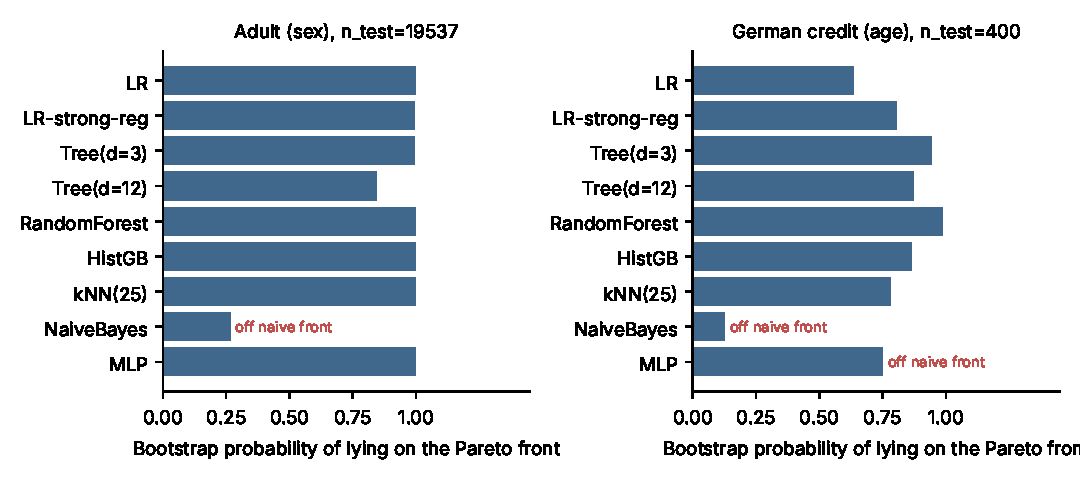
\includegraphics[width=0.9\textwidth]{fig_pareto_prob}
\caption{Bootstrap probability of Pareto-front membership. Labels mark models that are off the Pareto front of the point estimates.}\label{fig:pp}
\end{figure*}
\begin{figure*}[t]\centering
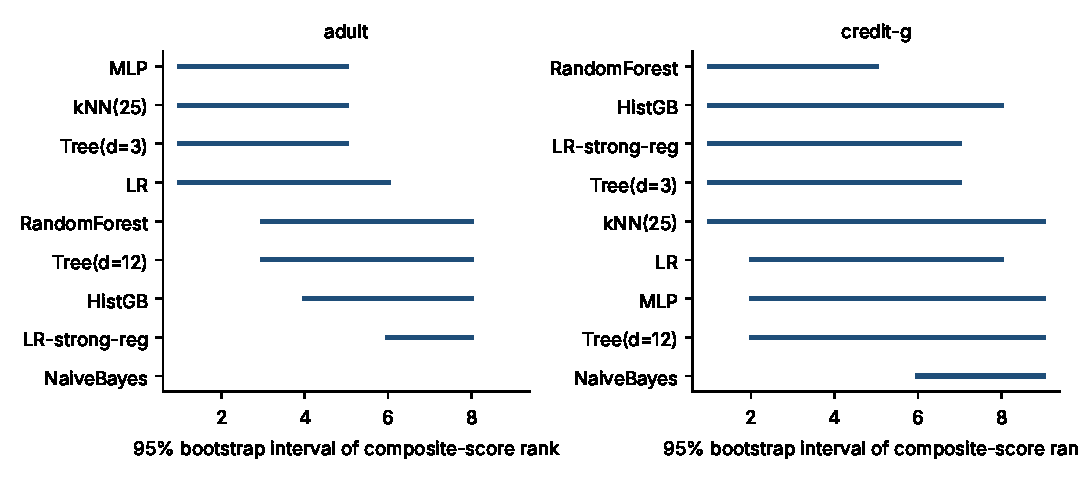
\includegraphics[width=0.9\textwidth]{fig_rank_intervals}
\caption{95\% bootstrap intervals for the rank of each model under the equal-weight composite score, models ordered by point-estimate rank.}\label{fig:rank}
\end{figure*}

\paragraph{Fewer criteria.} The TCS shrinks when fewer criteria are required (Table~\ref{tab:sub}), because dominance on fewer coordinates is easier to certify. With error and calibration only, Adult yields a TCS of five models against three on the naive front; with error and the equalised-odds gap it yields seven against two. On German credit no pair of criteria allows any exclusion. The naive front is never larger than the TCS, which illustrates the central point: the point-estimate front looks more decisive than the data warrant.

\begin{table}[t]\centering\footnotesize\setlength{\tabcolsep}{3pt}
\caption{Number of models retained, for each subset of criteria: TCS and the Pareto front of the point estimates (EO: equalised-odds gap; noise: noise drop).}\label{tab:sub}
\begin{tabular}{lrrrr}\toprule
Criteria subset & \multicolumn{2}{c}{Adult} & \multicolumn{2}{c}{German credit} \\
 & TCS & Naive & TCS & Naive \\\midrule
err + EO & 7 & 2 & 9 & 2 \\
err + ECE & 5 & 3 & 9 & 4 \\
err + noise & 7 & 6 & 9 & 3 \\
EO + ECE & 7 & 4 & 9 & 2 \\
EO + noise & 9 & 4 & 9 & 3 \\
ECE + noise & 7 & 3 & 9 & 4 \\
err + EO + ECE & 8 & 5 & 9 & 5 \\
err + EO + noise & 9 & 7 & 9 & 4 \\
err + ECE + noise & 7 & 7 & 9 & 6 \\
EO + ECE + noise & 9 & 6 & 9 & 5 \\
err + EO + ECE + noise & 9 & 8 & 9 & 7 \\
\bottomrule\end{tabular}
\end{table}

\section{Extensions}\label{sec:ext}
We examined four extensions. Details, code and caveats are in the repository (\texttt{docs/}); this section reports the results, including the null ones.

\paragraph{Step-down and a sharper critical value.} A step-down version in the style of Romano and Wolf \cite{romano2005} shrinks the family of tested models to the retained set at each step, and a two-stage preselection removes triples with very large statistics before computing the critical value (the latter is supported by a Bonferroni-split argument, not a full proof). In 300 replications per cell, every variant retained the nondominated set at least 98.7\% of the time. The step-down set was contained in the original TCS in all replications. The gain in exclusion was at most about one percentage point for step-down and two for preselection. On the two benchmarks no model was excluded under any variant: the largest dominance statistic is 0.59 on Adult and 0.51 on German credit, about three units below the critical value, so a sharper critical value cannot change the outcome.

\paragraph{Equivalence margin.} Excluding $m$ only when a rival is better by more than a margin $\varepsilon$ changes the target to the set $\mathcal{P}_0(\varepsilon)$ of models that are not $\varepsilon$-dominated, which contains $\mathcal{P}_0$. Retention of $\mathcal{P}_0(\varepsilon)$ was 0.997--1.000 in simulation for $\varepsilon\in\{0.01,0.02\}$, including the boundary case. The margin reduces the number of exclusions against $\mathcal{P}_0$ by construction, and the margin values here are illustrative only. Again no benchmark model was excluded.

\paragraph{Refit bootstrap.} Resampling only the test instances conditions on the trained models. We implemented a paired refit bootstrap (resample training and test rows independently, refit all models with a replicate-specific seed, evaluate on the resampled test rows), an out-of-bag variant and repeated random splits. The refit target is the learning algorithm averaged over training sets at the given size. On German credit ($n=1000$, 100 replicates) and a 4,000-row subsample of Adult (60 replicates), all nine models stayed in the set under every scheme; critical values rose from 3.71 to 4.63 (paired) and 5.10 (out-of-bag) on German credit. Pareto-membership probabilities and rank intervals moved much more than set membership: for the depth-12 tree on German credit the probability fell from 0.87 to 0.19. Bootstrap duplicates bias replicate means (error about 0.03 and ECE about 0.05 above the point estimate on German credit), and bootstrapping unstable learners is not guaranteed to be consistent. A simulation with a known truth (11 algorithms, three criteria) kept the population-nondominated algorithms in 100\% of replications for all schemes, but this is nearly uninformative because almost nothing was excluded, so calibration of the refit version remains untested. Repeated splits had the smallest spread in that simulation and may undercover.

\paragraph{Rank-graduation criteria.} Rank-based measures from the SAFE literature can be used as coordinates without change. We used 1$-$RGA (rank graduation accuracy, equal to $1-\mathrm{AUC}$ for a binary response), 1$-$RGR (rank graduation of predictions on clean against perturbed inputs) and the absolute difference of RGA between the two protected groups. The definitions were checked against a recent paper on rank graduation metrics \cite{auricchio2025} and the authors' software documentation; the original accuracy paper \cite{raffinetti2023} was available to us only as an abstract, the fairness coordinate follows the software rather than the binarised metric of Wu \cite{wu2026safe}, the explainability measure was not implemented, tie handling (mid-ranks) and the perturbation are our choices. On Adult these three criteria gave a TCS of eight of nine models, excluding logistic regression (statistic 3.44 against a critical value of 3.30), where the conventional four criteria retain all nine, and the Pareto-membership probability of logistic regression moved from 1.00 to 0.00. On German credit all nine models were retained under both criterion sets. The exclusion is a single model close to the threshold in a single split, so we treat it as an illustration that the choice of criteria changes the conclusion, not as a finding about logistic regression.

\section{Discussion}\label{sec:disc}
\paragraph{What the set says.} A TCS of size $M$ does not mean that all models are equally trustworthy. It means that, at the stated level, the test data do not contradict the claim that each is not strictly dominated. The practical consequences are that the choice among the retained models must rest on other grounds (cost, interpretability, domain constraints) and that, if a smaller set is wanted, one has to collect more test data, reduce the number of criteria or pre-specify a priority ordering.

\paragraph{Limitations.} (i) The main inference is conditional on the trained models and on one train/test split; retraining variance, seed variance and hyper-parameter search \cite{bouthillier2021,damour2022} are covered only by the refit extension, whose calibration we could not establish. The case studies use a single split and a single perturbation draw. (ii) Proposition~\ref{prop:cov} is an asymptotic statement under bootstrap consistency; criteria such as ECE with binning and the equalised-odds gap with a maximum are not smooth. The non-smooth simulation (Section~\ref{sec:nonsmooth}) showed no retention failure, but it covers four random designs and an estimator-matched population definition, and most of its cells exclude few models, so it is weak evidence about the nominal level. (iii) The procedure is conservative, as the simulation shows (retention above 99.7\% against a nominal 95\%) and costs power. (iv) The target is strict dominance; a model that is nearly dominated stays in $\mathcal{P}_0$. A practical-equivalence margin would be a useful refinement. (v) Candidate models are fixed in advance; selecting the list after looking at the test set invalidates the guarantee. (vi) The conceptual idea of a set-wise guarantee for the Pareto set of a finite list is not new (Section~\ref{sec:related}); what we claim is limited to the paired-bootstrap construction for functionals of a shared test sample and its use for trust criteria, and we did not search exhaustively. Two relevant papers (Arvanitis et al.\ and Jin et al.) were not read in full. (vii) The box comparison uses our own implementation, and the power gain depends on the correlation between models in the simulation design.

\paragraph{Extensions.} Natural directions are a theory-backed refit bootstrap, data-driven choices of equivalence margins, extension to explainability criteria such as attribution stability and to the binarised fairness measures of the SAFE family, and a comparison against the sequential procedures on a common benchmark.

\section*{Statements and Declarations}
\noindent\textbf{Funding.} None.\\
\textbf{Competing interests.} The author declares no competing interests.\\
\textbf{Data availability.} Both data sets are public (OpenML: Adult, version 2; credit-g, version 1).\\
\textbf{Code availability.} All code, simulation outputs and figures are in the repository accompanying this submission (directories \texttt{tcs}, \texttt{experiments}, \texttt{results}).

\begin{thebibliography}{99}
\bibitem{andradottir2021} Andrad{\'o}ttir S, Lee JS (2021) Pareto set estimation with guaranteed probability of correct selection. European Journal of Operational Research 292(1):286--298. \url{https://doi.org/10.1016/j.ejor.2020.10.021}
\bibitem{arvanitis2021} Arvanitis S, Post T, Poti V, Karabati S (2021) Nonparametric tests for optimal predictive ability. International Journal of Forecasting 37(2):881--898. \url{https://doi.org/10.1016/j.ijforecast.2020.10.002}
\bibitem{auer2016} Auer P, Chiang CK, Ortner R, Drugan M (2016) Pareto front identification from stochastic bandit feedback. Proceedings of the 19th International Conference on Artificial Intelligence and Statistics, PMLR 51:939--947
\bibitem{auerbach2024} Auerbach E, Liang A, Okumura K, Tabord-Meehan M (2024) Testing the fairness-accuracy improvability of algorithms. arXiv:2405.04816
\bibitem{auricchio2025} Auricchio G, Bernardelli AE, Giudici P, Toscani G (2025) On rank graduation metrics for high dimensional ordinal data. arXiv:2511.23100
\bibitem{crepon2024} Cr{\'e}pon E, Garivier A, Koolen WM (2024) Sequential learning of the Pareto front for multi-objective bandits. Proceedings of the 27th International Conference on Artificial Intelligence and Statistics, PMLR 238:3583--3591
\bibitem{jin2017} Jin S, Corradi V, Swanson NR (2017) Robust forecast comparison. Econometric Theory 33(6):1306--1351. \url{https://doi.org/10.1017/S0266466616000426}
\bibitem{kone2023} Kone C, Kaufmann E, Richert L (2023) Adaptive algorithms for relaxed Pareto set identification. Advances in Neural Information Processing Systems 36. arXiv:2307.00424
\bibitem{paretoinfer} Leite A, Ospina R, Ferraz C (2026) paretoinfer: sequential identification of approximately Pareto-optimal alternatives under noise. R package version 0.1.0. \url{https://cran.r-project.org/package=paretoinfer}
\bibitem{raffinetti2023} Raffinetti E (2023) A rank graduation accuracy measure to mitigate artificial intelligence risks. Quality \& Quantity 57:131--150. \url{https://doi.org/10.1007/s11135-023-01613-y}
\bibitem{zhao2026} Zhao J, Eckman DJ (2026) One-shot screening of simulated systems for acceptability. arXiv:2609.04400
\bibitem{babaei2025rgb} Babaei G, Giudici P, Raffinetti E (2025) A Rank Graduation Box for SAFE AI. Expert Systems with Applications 259:125239. \url{https://doi.org/10.1016/j.eswa.2024.125239}
\bibitem{benavoli2017} Benavoli A, Corani G, Dem{\v s}ar J, Zaffalon M (2017) Time for a change: a tutorial for comparing multiple classifiers through Bayesian analysis. Journal of Machine Learning Research 18(77):1--36
\bibitem{bouthillier2021} Bouthillier X, Delaunay P, Bronzi M, et al. (2021) Accounting for variance in machine learning benchmarks. Proceedings of Machine Learning and Systems 3. arXiv:2103.03098
\bibitem{damour2022} D'Amour A, Heller K, Moldovan D, et al. (2022) Underspecification presents challenges for credibility in modern machine learning. Journal of Machine Learning Research 23(226):1--61. arXiv:2011.03395
\bibitem{demsar2006} Dem{\v s}ar J (2006) Statistical comparisons of classifiers over multiple data sets. Journal of Machine Learning Research 7:1--30
\bibitem{dietterich1998} Dietterich TG (1998) Approximate statistical tests for comparing supervised classification learning algorithms. Neural Computation 10(7):1895--1923. \url{https://doi.org/10.1162/089976698300017197}
\bibitem{ferrara2025} Ferrara A, Cozzi F, Perotti A, et al. (2025) Size-adaptive hypothesis testing for fairness. Advances in Neural Information Processing Systems 38. arXiv:2506.10586
\bibitem{giudici2024robust} Giudici P, Raffinetti E, Riani M (2024) Robust machine learning models: linear and nonlinear. International Journal of Data Science and Analytics 20:1043--1050. \url{https://doi.org/10.1007/s41060-024-00512-1}
\bibitem{guo2017} Guo C, Pleiss G, Sun Y, Weinberger KQ (2017) On calibration of modern neural networks. Proceedings of the 34th International Conference on Machine Learning. arXiv:1706.04599
\bibitem{hansen2005spa} Hansen PR (2005) A test for superior predictive ability. Journal of Business \& Economic Statistics 23(4):365--380. \url{https://doi.org/10.1198/073500105000000063}
\bibitem{hansen2011mcs} Hansen PR, Lunde A, Nason JM (2011) The model confidence set. Econometrica 79(2):453--497. \url{https://doi.org/10.3982/ECTA5771}
\bibitem{hardt2016} Hardt M, Price E, Srebro N (2016) Equality of opportunity in supervised learning. Advances in Neural Information Processing Systems 29. arXiv:1610.02413
\bibitem{marx2020} Marx CT, Calmon FP, Ustun B (2020) Predictive multiplicity in classification. Proceedings of the 37th International Conference on Machine Learning. arXiv:1909.06677
\bibitem{miller2021} Miller AC, Gatys LA, Futoma J, Fox EB (2021) Model-based metrics: sample-efficient estimates of predictive model subpopulation performance. Proceedings of Machine Learning Research 149 (MLHC 2021)
\bibitem{nikitina2026} Nikitina E, Mouri{\~n}o H (2026) Reconstruction accuracy versus predictive performance: evaluating imputation methods under real-world missingness. International Journal of Data Science and Analytics 22:362. \url{https://doi.org/10.1007/s41060-026-01295-3}
\bibitem{romano2005} Romano JP, Wolf M (2005) Stepwise multiple testing as formalized data snooping. Econometrica 73(4):1237--1282. \url{https://doi.org/10.1111/j.1468-0262.2005.00615.x}
\bibitem{white2000} White H (2000) A reality check for data snooping. Econometrica 68(5):1097--1126. \url{https://doi.org/10.1111/1468-0262.00152}
\bibitem{wu2026safe} Wu L (2026) Evaluating credit lending fairness with binarized continuous variables in SAFE metrics. International Journal of Data Science and Analytics 22. \url{https://doi.org/10.1007/s41060-025-01002-8}
\bibitem{zhang2018sprint} Zhang T, Georgiopoulos M, Anagnostopoulos GC (2018) Pareto-optimal model selection via SPRINT-Race. IEEE Transactions on Cybernetics 48(2):596--610. \url{https://doi.org/10.1109/TCYB.2017.2647821}
\end{thebibliography}
\end{document}
